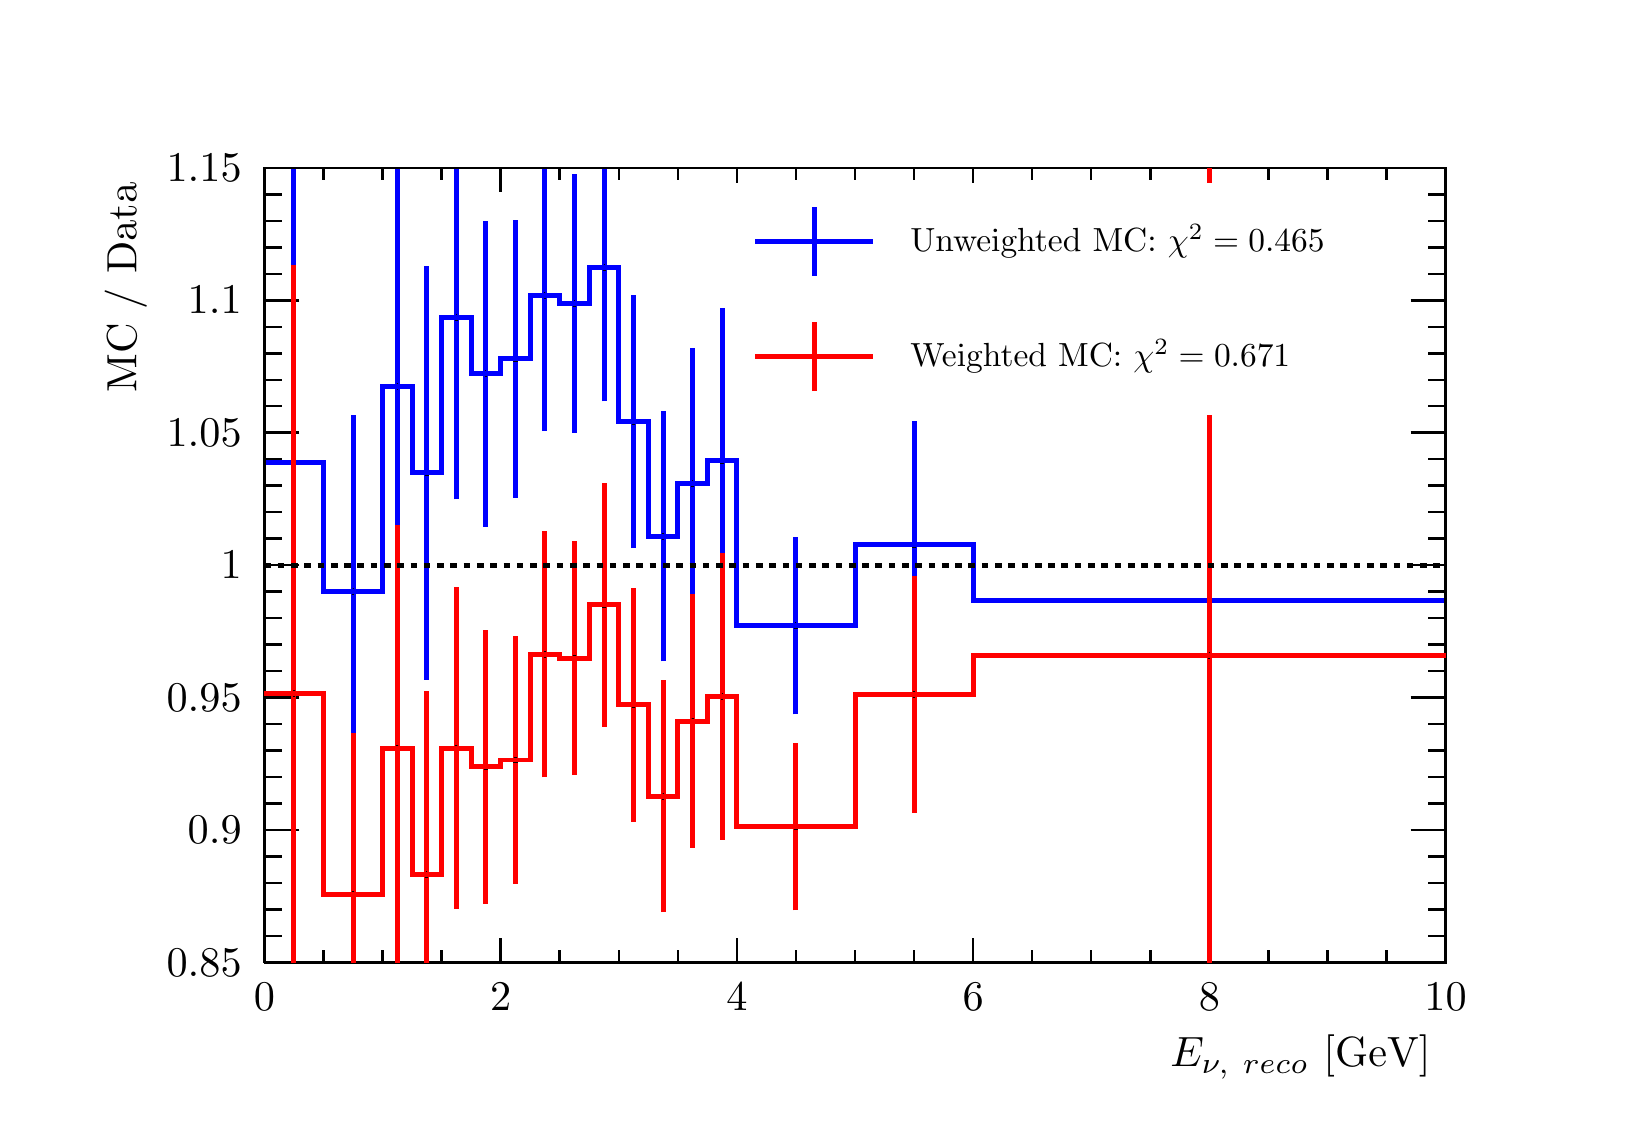
\begin{tikzpicture}
\pgfdeclareplotmark{cross} {
\pgfpathmoveto{\pgfpoint{-0.3\pgfplotmarksize}{\pgfplotmarksize}}
\pgfpathlineto{\pgfpoint{+0.3\pgfplotmarksize}{\pgfplotmarksize}}
\pgfpathlineto{\pgfpoint{+0.3\pgfplotmarksize}{0.3\pgfplotmarksize}}
\pgfpathlineto{\pgfpoint{+1\pgfplotmarksize}{0.3\pgfplotmarksize}}
\pgfpathlineto{\pgfpoint{+1\pgfplotmarksize}{-0.3\pgfplotmarksize}}
\pgfpathlineto{\pgfpoint{+0.3\pgfplotmarksize}{-0.3\pgfplotmarksize}}
\pgfpathlineto{\pgfpoint{+0.3\pgfplotmarksize}{-1.\pgfplotmarksize}}
\pgfpathlineto{\pgfpoint{-0.3\pgfplotmarksize}{-1.\pgfplotmarksize}}
\pgfpathlineto{\pgfpoint{-0.3\pgfplotmarksize}{-0.3\pgfplotmarksize}}
\pgfpathlineto{\pgfpoint{-1.\pgfplotmarksize}{-0.3\pgfplotmarksize}}
\pgfpathlineto{\pgfpoint{-1.\pgfplotmarksize}{0.3\pgfplotmarksize}}
\pgfpathlineto{\pgfpoint{-0.3\pgfplotmarksize}{0.3\pgfplotmarksize}}
\pgfpathclose
\pgfusepathqstroke
}
\pgfdeclareplotmark{cross*} {
\pgfpathmoveto{\pgfpoint{-0.3\pgfplotmarksize}{\pgfplotmarksize}}
\pgfpathlineto{\pgfpoint{+0.3\pgfplotmarksize}{\pgfplotmarksize}}
\pgfpathlineto{\pgfpoint{+0.3\pgfplotmarksize}{0.3\pgfplotmarksize}}
\pgfpathlineto{\pgfpoint{+1\pgfplotmarksize}{0.3\pgfplotmarksize}}
\pgfpathlineto{\pgfpoint{+1\pgfplotmarksize}{-0.3\pgfplotmarksize}}
\pgfpathlineto{\pgfpoint{+0.3\pgfplotmarksize}{-0.3\pgfplotmarksize}}
\pgfpathlineto{\pgfpoint{+0.3\pgfplotmarksize}{-1.\pgfplotmarksize}}
\pgfpathlineto{\pgfpoint{-0.3\pgfplotmarksize}{-1.\pgfplotmarksize}}
\pgfpathlineto{\pgfpoint{-0.3\pgfplotmarksize}{-0.3\pgfplotmarksize}}
\pgfpathlineto{\pgfpoint{-1.\pgfplotmarksize}{-0.3\pgfplotmarksize}}
\pgfpathlineto{\pgfpoint{-1.\pgfplotmarksize}{0.3\pgfplotmarksize}}
\pgfpathlineto{\pgfpoint{-0.3\pgfplotmarksize}{0.3\pgfplotmarksize}}
\pgfpathclose
\pgfusepathqfillstroke
}
\pgfdeclareplotmark{newstar} {
\pgfpathmoveto{\pgfqpoint{0pt}{\pgfplotmarksize}}
\pgfpathlineto{\pgfqpointpolar{44}{0.5\pgfplotmarksize}}
\pgfpathlineto{\pgfqpointpolar{18}{\pgfplotmarksize}}
\pgfpathlineto{\pgfqpointpolar{-20}{0.5\pgfplotmarksize}}
\pgfpathlineto{\pgfqpointpolar{-54}{\pgfplotmarksize}}
\pgfpathlineto{\pgfqpointpolar{-90}{0.5\pgfplotmarksize}}
\pgfpathlineto{\pgfqpointpolar{234}{\pgfplotmarksize}}
\pgfpathlineto{\pgfqpointpolar{198}{0.5\pgfplotmarksize}}
\pgfpathlineto{\pgfqpointpolar{162}{\pgfplotmarksize}}
\pgfpathlineto{\pgfqpointpolar{134}{0.5\pgfplotmarksize}}
\pgfpathclose
\pgfusepathqstroke
}
\pgfdeclareplotmark{newstar*} {
\pgfpathmoveto{\pgfqpoint{0pt}{\pgfplotmarksize}}
\pgfpathlineto{\pgfqpointpolar{44}{0.5\pgfplotmarksize}}
\pgfpathlineto{\pgfqpointpolar{18}{\pgfplotmarksize}}
\pgfpathlineto{\pgfqpointpolar{-20}{0.5\pgfplotmarksize}}
\pgfpathlineto{\pgfqpointpolar{-54}{\pgfplotmarksize}}
\pgfpathlineto{\pgfqpointpolar{-90}{0.5\pgfplotmarksize}}
\pgfpathlineto{\pgfqpointpolar{234}{\pgfplotmarksize}}
\pgfpathlineto{\pgfqpointpolar{198}{0.5\pgfplotmarksize}}
\pgfpathlineto{\pgfqpointpolar{162}{\pgfplotmarksize}}
\pgfpathlineto{\pgfqpointpolar{134}{0.5\pgfplotmarksize}}
\pgfpathclose
\pgfusepathqfillstroke
}
\definecolor{c}{rgb}{1,1,1};
\draw [color=c, fill=c] (0,0) rectangle (20,13.639);
\draw [color=c, fill=c] (3,1.77307) rectangle (18,11.8659);
\definecolor{c}{rgb}{0,0,0};
\draw [c,line width=0.9] (3,1.77307) -- (3,11.8659) -- (18,11.8659) -- (18,1.77307) -- (3,1.77307);
\definecolor{c}{rgb}{1,1,1};
\draw [color=c, fill=c] (3,1.77307) rectangle (18,11.8659);
\definecolor{c}{rgb}{0,0,0};
\draw [c,line width=0.9] (3,1.77307) -- (3,11.8659) -- (18,11.8659) -- (18,1.77307) -- (3,1.77307);
\definecolor{c}{rgb}{0,0,1};
\draw [c,line width=1.8] (3.375,2.31426) -- (3.375,8.12556);
\draw [c,line width=1.8] (3.375,8.12556) -- (3.375,11.8659);
\definecolor{c}{rgb}{0,0,0};
\foreach \P in {(3.375,8.12556)}{\draw[mark options={color=c,fill=c},mark size=2.402402pt, line width=0.000000pt, mark=*,mark size=1pt] plot coordinates {\P};}
\definecolor{c}{rgb}{0,0,1};
\draw [c,line width=1.8] (4.125,4.2494) -- (4.125,6.48732);
\draw [c,line width=1.8] (4.125,6.48732) -- (4.125,8.72525);
\definecolor{c}{rgb}{0,0,0};
\foreach \P in {(4.125,6.48732)}{\draw[mark options={color=c,fill=c},mark size=2.402402pt, line width=0.000000pt, mark=*,mark size=1pt] plot coordinates {\P};}
\definecolor{c}{rgb}{0,0,1};
\draw [c,line width=1.8] (4.6875,5.94758) -- (4.6875,9.09073);
\draw [c,line width=1.8] (4.6875,9.09073) -- (4.6875,11.8659);
\definecolor{c}{rgb}{0,0,0};
\foreach \P in {(4.6875,9.09073)}{\draw[mark options={color=c,fill=c},mark size=2.402402pt, line width=0.000000pt, mark=*,mark size=1pt] plot coordinates {\P};}
\definecolor{c}{rgb}{0,0,1};
\draw [c,line width=1.8] (5.0625,5.36325) -- (5.0625,7.99115);
\draw [c,line width=1.8] (5.0625,7.99115) -- (5.0625,10.619);
\definecolor{c}{rgb}{0,0,0};
\foreach \P in {(5.0625,7.99115)}{\draw[mark options={color=c,fill=c},mark size=2.402402pt, line width=0.000000pt, mark=*,mark size=1pt] plot coordinates {\P};}
\definecolor{c}{rgb}{0,0,1};
\draw [c,line width=1.8] (5.4375,7.65638) -- (5.4375,9.96416);
\draw [c,line width=1.8] (5.4375,9.96416) -- (5.4375,11.8659);
\definecolor{c}{rgb}{0,0,0};
\foreach \P in {(5.4375,9.96416)}{\draw[mark options={color=c,fill=c},mark size=2.402402pt, line width=0.000000pt, mark=*,mark size=1pt] plot coordinates {\P};}
\definecolor{c}{rgb}{0,0,1};
\draw [c,line width=1.8] (5.8125,7.30917) -- (5.8125,9.25287);
\draw [c,line width=1.8] (5.8125,9.25287) -- (5.8125,11.1966);
\definecolor{c}{rgb}{0,0,0};
\foreach \P in {(5.8125,9.25287)}{\draw[mark options={color=c,fill=c},mark size=2.402402pt, line width=0.000000pt, mark=*,mark size=1pt] plot coordinates {\P};}
\definecolor{c}{rgb}{0,0,1};
\draw [c,line width=1.8] (6.1875,7.67831) -- (6.1875,9.43954);
\draw [c,line width=1.8] (6.1875,9.43954) -- (6.1875,11.2008);
\definecolor{c}{rgb}{0,0,0};
\foreach \P in {(6.1875,9.43954)}{\draw[mark options={color=c,fill=c},mark size=2.402402pt, line width=0.000000pt, mark=*,mark size=1pt] plot coordinates {\P};}
\definecolor{c}{rgb}{0,0,1};
\draw [c,line width=1.8] (6.5625,8.52126) -- (6.5625,10.245);
\draw [c,line width=1.8] (6.5625,10.245) -- (6.5625,11.8659);
\definecolor{c}{rgb}{0,0,0};
\foreach \P in {(6.5625,10.245)}{\draw[mark options={color=c,fill=c},mark size=2.402402pt, line width=0.000000pt, mark=*,mark size=1pt] plot coordinates {\P};}
\definecolor{c}{rgb}{0,0,1};
\draw [c,line width=1.8] (6.9375,8.50207) -- (6.9375,10.1425);
\draw [c,line width=1.8] (6.9375,10.1425) -- (6.9375,11.7828);
\definecolor{c}{rgb}{0,0,0};
\foreach \P in {(6.9375,10.1425)}{\draw[mark options={color=c,fill=c},mark size=2.402402pt, line width=0.000000pt, mark=*,mark size=1pt] plot coordinates {\P};}
\definecolor{c}{rgb}{0,0,1};
\draw [c,line width=1.8] (7.3125,8.90128) -- (7.3125,10.5982);
\draw [c,line width=1.8] (7.3125,10.5982) -- (7.3125,11.8659);
\definecolor{c}{rgb}{0,0,0};
\foreach \P in {(7.3125,10.5982)}{\draw[mark options={color=c,fill=c},mark size=2.402402pt, line width=0.000000pt, mark=*,mark size=1pt] plot coordinates {\P};}
\definecolor{c}{rgb}{0,0,1};
\draw [c,line width=1.8] (7.6875,7.03483) -- (7.6875,8.6408);
\draw [c,line width=1.8] (7.6875,8.6408) -- (7.6875,10.2468);
\definecolor{c}{rgb}{0,0,0};
\foreach \P in {(7.6875,8.6408)}{\draw[mark options={color=c,fill=c},mark size=2.402402pt, line width=0.000000pt, mark=*,mark size=1pt] plot coordinates {\P};}
\definecolor{c}{rgb}{0,0,1};
\draw [c,line width=1.8] (8.0625,5.59828) -- (8.0625,7.18646);
\draw [c,line width=1.8] (8.0625,7.18646) -- (8.0625,8.77463);
\definecolor{c}{rgb}{0,0,0};
\foreach \P in {(8.0625,7.18646)}{\draw[mark options={color=c,fill=c},mark size=2.402402pt, line width=0.000000pt, mark=*,mark size=1pt] plot coordinates {\P};}
\definecolor{c}{rgb}{0,0,1};
\draw [c,line width=1.8] (8.4375,6.13448) -- (8.4375,7.85667);
\draw [c,line width=1.8] (8.4375,7.85667) -- (8.4375,9.57886);
\definecolor{c}{rgb}{0,0,0};
\foreach \P in {(8.4375,7.85667)}{\draw[mark options={color=c,fill=c},mark size=2.402402pt, line width=0.000000pt, mark=*,mark size=1pt] plot coordinates {\P};}
\definecolor{c}{rgb}{0,0,1};
\draw [c,line width=1.8] (8.8125,6.19975) -- (8.8125,8.14559);
\draw [c,line width=1.8] (8.8125,8.14559) -- (8.8125,10.0914);
\definecolor{c}{rgb}{0,0,0};
\foreach \P in {(8.8125,8.14559)}{\draw[mark options={color=c,fill=c},mark size=2.402402pt, line width=0.000000pt, mark=*,mark size=1pt] plot coordinates {\P};}
\definecolor{c}{rgb}{0,0,1};
\draw [c,line width=1.8] (9.75,4.92583) -- (9.75,6.05061);
\draw [c,line width=1.8] (9.75,6.05061) -- (9.75,7.1754);
\definecolor{c}{rgb}{0,0,0};
\foreach \P in {(9.75,6.05061)}{\draw[mark options={color=c,fill=c},mark size=2.402402pt, line width=0.000000pt, mark=*,mark size=1pt] plot coordinates {\P};}
\definecolor{c}{rgb}{0,0,1};
\draw [c,line width=1.8] (11.25,5.50278) -- (11.25,7.07607);
\draw [c,line width=1.8] (11.25,7.07607) -- (11.25,8.64936);
\definecolor{c}{rgb}{0,0,0};
\foreach \P in {(11.25,7.07607)}{\draw[mark options={color=c,fill=c},mark size=2.402402pt, line width=0.000000pt, mark=*,mark size=1pt] plot coordinates {\P};}
\definecolor{c}{rgb}{0,0,1};
\draw [c,line width=1.8] (15,1.77307) -- (15,6.3769);
\draw [c,line width=1.8] (15,6.3769) -- (15,11.8659);
\definecolor{c}{rgb}{0,0,0};
\foreach \P in {(15,6.3769)}{\draw[mark options={color=c,fill=c},mark size=2.402402pt, line width=0.000000pt, mark=*,mark size=1pt] plot coordinates {\P};}
\definecolor{c}{rgb}{0,0,1};
\draw [c,line width=1.8] (3,8.12556) -- (3.75,8.12556) -- (3.75,6.48732) -- (4.5,6.48732) -- (4.5,9.09073) -- (4.875,9.09073) -- (4.875,7.99115) -- (5.25,7.99115) -- (5.25,9.96416) -- (5.625,9.96416) -- (5.625,9.25287) -- (6,9.25287) -- (6,9.43954)
 -- (6.375,9.43954) -- (6.375,10.245) -- (6.75,10.245) -- (6.75,10.1425) -- (7.125,10.1425) -- (7.125,10.5982) -- (7.5,10.5982) -- (7.5,8.6408) -- (7.875,8.6408) -- (7.875,7.18646) -- (8.25,7.18646) -- (8.25,7.85667) -- (8.625,7.85667) --
 (8.625,8.14559) -- (9,8.14559) -- (9,6.05061) -- (10.5,6.05061) -- (10.5,7.07607) -- (12,7.07607) -- (12,6.3769) -- (18,6.3769);
\definecolor{c}{rgb}{0,0,0};
\draw [c,line width=0.9] (3,1.77307) -- (18,1.77307);
\draw [c,line width=0.9] (3,2.07994) -- (3,1.77307);
\draw [c,line width=0.9] (3.75,1.9265) -- (3.75,1.77307);
\draw [c,line width=0.9] (4.5,1.9265) -- (4.5,1.77307);
\draw [c,line width=0.9] (5.25,1.9265) -- (5.25,1.77307);
\draw [c,line width=0.9] (6,2.07994) -- (6,1.77307);
\draw [c,line width=0.9] (6.75,1.9265) -- (6.75,1.77307);
\draw [c,line width=0.9] (7.5,1.9265) -- (7.5,1.77307);
\draw [c,line width=0.9] (8.25,1.9265) -- (8.25,1.77307);
\draw [c,line width=0.9] (9,2.07994) -- (9,1.77307);
\draw [c,line width=0.9] (9.75,1.9265) -- (9.75,1.77307);
\draw [c,line width=0.9] (10.5,1.9265) -- (10.5,1.77307);
\draw [c,line width=0.9] (11.25,1.9265) -- (11.25,1.77307);
\draw [c,line width=0.9] (12,2.07994) -- (12,1.77307);
\draw [c,line width=0.9] (12.75,1.9265) -- (12.75,1.77307);
\draw [c,line width=0.9] (13.5,1.9265) -- (13.5,1.77307);
\draw [c,line width=0.9] (14.25,1.9265) -- (14.25,1.77307);
\draw [c,line width=0.9] (15,2.07994) -- (15,1.77307);
\draw [c,line width=0.9] (15.75,1.9265) -- (15.75,1.77307);
\draw [c,line width=0.9] (16.5,1.9265) -- (16.5,1.77307);
\draw [c,line width=0.9] (17.25,1.9265) -- (17.25,1.77307);
\draw [c,line width=0.9] (18,2.07994) -- (18,1.77307);
\draw [anchor=base] (3,1.15931) node[scale=1.52731, color=c, rotate=0]{0};
\draw [anchor=base] (6,1.15931) node[scale=1.52731, color=c, rotate=0]{2};
\draw [anchor=base] (9,1.15931) node[scale=1.52731, color=c, rotate=0]{4};
\draw [anchor=base] (12,1.15931) node[scale=1.52731, color=c, rotate=0]{6};
\draw [anchor=base] (15,1.15931) node[scale=1.52731, color=c, rotate=0]{8};
\draw [anchor=base] (18,1.15931) node[scale=1.52731, color=c, rotate=0]{10};
\draw [anchor= east] (18,0.572837) node[scale=1.52731, color=c, rotate=0]{$E_{\nu,~\text{reco}}$ [GeV]};
\draw [c,line width=0.9] (3,11.8659) -- (18,11.8659);
\draw [c,line width=0.9] (3,11.559) -- (3,11.8659);
\draw [c,line width=0.9] (3.75,11.7125) -- (3.75,11.8659);
\draw [c,line width=0.9] (4.5,11.7125) -- (4.5,11.8659);
\draw [c,line width=0.9] (5.25,11.7125) -- (5.25,11.8659);
\draw [c,line width=0.9] (6,11.559) -- (6,11.8659);
\draw [c,line width=0.9] (6.75,11.7125) -- (6.75,11.8659);
\draw [c,line width=0.9] (7.5,11.7125) -- (7.5,11.8659);
\draw [c,line width=0.9] (8.25,11.7125) -- (8.25,11.8659);
\draw [c,line width=0.9] (9,11.559) -- (9,11.8659);
\draw [c,line width=0.9] (9.75,11.7125) -- (9.75,11.8659);
\draw [c,line width=0.9] (10.5,11.7125) -- (10.5,11.8659);
\draw [c,line width=0.9] (11.25,11.7125) -- (11.25,11.8659);
\draw [c,line width=0.9] (12,11.559) -- (12,11.8659);
\draw [c,line width=0.9] (12.75,11.7125) -- (12.75,11.8659);
\draw [c,line width=0.9] (13.5,11.7125) -- (13.5,11.8659);
\draw [c,line width=0.9] (14.25,11.7125) -- (14.25,11.8659);
\draw [c,line width=0.9] (15,11.559) -- (15,11.8659);
\draw [c,line width=0.9] (15.75,11.7125) -- (15.75,11.8659);
\draw [c,line width=0.9] (16.5,11.7125) -- (16.5,11.8659);
\draw [c,line width=0.9] (17.25,11.7125) -- (17.25,11.8659);
\draw [c,line width=0.9] (18,11.559) -- (18,11.8659);
\draw [c,line width=0.9] (3,1.77307) -- (3,11.8659);
\draw [c,line width=0.9] (3.444,1.77307) -- (3,1.77307);
\draw [c,line width=0.9] (3.222,2.10949) -- (3,2.10949);
\draw [c,line width=0.9] (3.222,2.44592) -- (3,2.44592);
\draw [c,line width=0.9] (3.222,2.78235) -- (3,2.78235);
\draw [c,line width=0.9] (3.222,3.11878) -- (3,3.11878);
\draw [c,line width=0.9] (3.444,3.45521) -- (3,3.45521);
\draw [c,line width=0.9] (3.222,3.79163) -- (3,3.79163);
\draw [c,line width=0.9] (3.222,4.12806) -- (3,4.12806);
\draw [c,line width=0.9] (3.222,4.46449) -- (3,4.46449);
\draw [c,line width=0.9] (3.222,4.80092) -- (3,4.80092);
\draw [c,line width=0.9] (3.444,5.13734) -- (3,5.13734);
\draw [c,line width=0.9] (3.222,5.47377) -- (3,5.47377);
\draw [c,line width=0.9] (3.222,5.8102) -- (3,5.8102);
\draw [c,line width=0.9] (3.222,6.14663) -- (3,6.14663);
\draw [c,line width=0.9] (3.222,6.48306) -- (3,6.48306);
\draw [c,line width=0.9] (3.444,6.81948) -- (3,6.81948);
\draw [c,line width=0.9] (3.222,7.15591) -- (3,7.15591);
\draw [c,line width=0.9] (3.222,7.49234) -- (3,7.49234);
\draw [c,line width=0.9] (3.222,7.82877) -- (3,7.82877);
\draw [c,line width=0.9] (3.222,8.1652) -- (3,8.1652);
\draw [c,line width=0.9] (3.444,8.50162) -- (3,8.50162);
\draw [c,line width=0.9] (3.222,8.83805) -- (3,8.83805);
\draw [c,line width=0.9] (3.222,9.17448) -- (3,9.17448);
\draw [c,line width=0.9] (3.222,9.51091) -- (3,9.51091);
\draw [c,line width=0.9] (3.222,9.84733) -- (3,9.84733);
\draw [c,line width=0.9] (3.444,10.1838) -- (3,10.1838);
\draw [c,line width=0.9] (3.222,10.5202) -- (3,10.5202);
\draw [c,line width=0.9] (3.222,10.8566) -- (3,10.8566);
\draw [c,line width=0.9] (3.222,11.193) -- (3,11.193);
\draw [c,line width=0.9] (3.222,11.5295) -- (3,11.5295);
\draw [c,line width=0.9] (3.444,11.8659) -- (3,11.8659);
\draw [c,line width=0.9] (3.444,1.77307) -- (3,1.77307);
\draw [c,line width=0.9] (3.444,11.8659) -- (3,11.8659);
\draw [anchor= east] (2.9,1.77307) node[scale=1.52731, color=c, rotate=0]{0.85};
\draw [anchor= east] (2.9,3.45521) node[scale=1.52731, color=c, rotate=0]{0.9};
\draw [anchor= east] (2.9,5.13734) node[scale=1.52731, color=c, rotate=0]{0.95};
\draw [anchor= east] (2.9,6.81948) node[scale=1.52731, color=c, rotate=0]{1};
\draw [anchor= east] (2.9,8.50162) node[scale=1.52731, color=c, rotate=0]{1.05};
\draw [anchor= east] (2.9,10.1838) node[scale=1.52731, color=c, rotate=0]{1.1};
\draw [anchor= east] (2.9,11.8659) node[scale=1.52731, color=c, rotate=0]{1.15};
\draw [anchor= east] (1.24,11.8659) node[scale=1.52731, color=c, rotate=90]{MC / Data};
\draw [c,line width=0.9] (18,1.77307) -- (18,11.8659);
\draw [c,line width=0.9] (17.556,1.77307) -- (18,1.77307);
\draw [c,line width=0.9] (17.778,2.10949) -- (18,2.10949);
\draw [c,line width=0.9] (17.778,2.44592) -- (18,2.44592);
\draw [c,line width=0.9] (17.778,2.78235) -- (18,2.78235);
\draw [c,line width=0.9] (17.778,3.11878) -- (18,3.11878);
\draw [c,line width=0.9] (17.556,3.45521) -- (18,3.45521);
\draw [c,line width=0.9] (17.778,3.79163) -- (18,3.79163);
\draw [c,line width=0.9] (17.778,4.12806) -- (18,4.12806);
\draw [c,line width=0.9] (17.778,4.46449) -- (18,4.46449);
\draw [c,line width=0.9] (17.778,4.80092) -- (18,4.80092);
\draw [c,line width=0.9] (17.556,5.13734) -- (18,5.13734);
\draw [c,line width=0.9] (17.778,5.47377) -- (18,5.47377);
\draw [c,line width=0.9] (17.778,5.8102) -- (18,5.8102);
\draw [c,line width=0.9] (17.778,6.14663) -- (18,6.14663);
\draw [c,line width=0.9] (17.778,6.48306) -- (18,6.48306);
\draw [c,line width=0.9] (17.556,6.81948) -- (18,6.81948);
\draw [c,line width=0.9] (17.778,7.15591) -- (18,7.15591);
\draw [c,line width=0.9] (17.778,7.49234) -- (18,7.49234);
\draw [c,line width=0.9] (17.778,7.82877) -- (18,7.82877);
\draw [c,line width=0.9] (17.778,8.1652) -- (18,8.1652);
\draw [c,line width=0.9] (17.556,8.50162) -- (18,8.50162);
\draw [c,line width=0.9] (17.778,8.83805) -- (18,8.83805);
\draw [c,line width=0.9] (17.778,9.17448) -- (18,9.17448);
\draw [c,line width=0.9] (17.778,9.51091) -- (18,9.51091);
\draw [c,line width=0.9] (17.778,9.84733) -- (18,9.84733);
\draw [c,line width=0.9] (17.556,10.1838) -- (18,10.1838);
\draw [c,line width=0.9] (17.778,10.5202) -- (18,10.5202);
\draw [c,line width=0.9] (17.778,10.8566) -- (18,10.8566);
\draw [c,line width=0.9] (17.778,11.193) -- (18,11.193);
\draw [c,line width=0.9] (17.778,11.5295) -- (18,11.5295);
\draw [c,line width=0.9] (17.556,11.8659) -- (18,11.8659);
\draw [c,line width=0.9] (17.556,1.77307) -- (18,1.77307);
\draw [c,line width=0.9] (17.556,11.8659) -- (18,11.8659);
\definecolor{c}{rgb}{1,0,0};
\draw [c,line width=1.8] (3.375,1.77307) -- (3.375,5.19287);
\draw [c,line width=1.8] (3.375,5.19287) -- (3.375,10.6348);
\definecolor{c}{rgb}{0,0,0};
\foreach \P in {(3.375,5.19287)}{\draw[mark options={color=c,fill=c},mark size=2.402402pt, line width=0.000000pt, mark=*,mark size=1pt] plot coordinates {\P};}
\definecolor{c}{rgb}{1,0,0};
\draw [c,line width=1.8] (4.125,1.77307) -- (4.125,2.64138);
\draw [c,line width=1.8] (4.125,2.64138) -- (4.125,4.6848);
\definecolor{c}{rgb}{0,0,0};
\foreach \P in {(4.125,2.64138)}{\draw[mark options={color=c,fill=c},mark size=2.402402pt, line width=0.000000pt, mark=*,mark size=1pt] plot coordinates {\P};}
\definecolor{c}{rgb}{1,0,0};
\draw [c,line width=1.8] (4.6875,1.77307) -- (4.6875,4.49591);
\draw [c,line width=1.8] (4.6875,4.49591) -- (4.6875,7.33251);
\definecolor{c}{rgb}{0,0,0};
\foreach \P in {(4.6875,4.49591)}{\draw[mark options={color=c,fill=c},mark size=2.402402pt, line width=0.000000pt, mark=*,mark size=1pt] plot coordinates {\P};}
\definecolor{c}{rgb}{1,0,0};
\draw [c,line width=1.8] (5.0625,1.77307) -- (5.0625,2.88941);
\draw [c,line width=1.8] (5.0625,2.88941) -- (5.0625,5.22492);
\definecolor{c}{rgb}{0,0,0};
\foreach \P in {(5.0625,2.88941)}{\draw[mark options={color=c,fill=c},mark size=2.402402pt, line width=0.000000pt, mark=*,mark size=1pt] plot coordinates {\P};}
\definecolor{c}{rgb}{1,0,0};
\draw [c,line width=1.8] (5.4375,2.45044) -- (5.4375,4.49544);
\draw [c,line width=1.8] (5.4375,4.49544) -- (5.4375,6.54045);
\definecolor{c}{rgb}{0,0,0};
\foreach \P in {(5.4375,4.49544)}{\draw[mark options={color=c,fill=c},mark size=2.402402pt, line width=0.000000pt, mark=*,mark size=1pt] plot coordinates {\P};}
\definecolor{c}{rgb}{1,0,0};
\draw [c,line width=1.8] (5.8125,2.51887) -- (5.8125,4.25714);
\draw [c,line width=1.8] (5.8125,4.25714) -- (5.8125,5.99541);
\definecolor{c}{rgb}{0,0,0};
\foreach \P in {(5.8125,4.25714)}{\draw[mark options={color=c,fill=c},mark size=2.402402pt, line width=0.000000pt, mark=*,mark size=1pt] plot coordinates {\P};}
\definecolor{c}{rgb}{1,0,0};
\draw [c,line width=1.8] (6.1875,2.77331) -- (6.1875,4.34554);
\draw [c,line width=1.8] (6.1875,4.34554) -- (6.1875,5.91776);
\definecolor{c}{rgb}{0,0,0};
\foreach \P in {(6.1875,4.34554)}{\draw[mark options={color=c,fill=c},mark size=2.402402pt, line width=0.000000pt, mark=*,mark size=1pt] plot coordinates {\P};}
\definecolor{c}{rgb}{1,0,0};
\draw [c,line width=1.8] (6.5625,4.12631) -- (6.5625,5.68777);
\draw [c,line width=1.8] (6.5625,5.68777) -- (6.5625,7.24923);
\definecolor{c}{rgb}{0,0,0};
\foreach \P in {(6.5625,5.68777)}{\draw[mark options={color=c,fill=c},mark size=2.402402pt, line width=0.000000pt, mark=*,mark size=1pt] plot coordinates {\P};}
\definecolor{c}{rgb}{1,0,0};
\draw [c,line width=1.8] (6.9375,4.15287) -- (6.9375,5.6403);
\draw [c,line width=1.8] (6.9375,5.6403) -- (6.9375,7.12773);
\definecolor{c}{rgb}{0,0,0};
\foreach \P in {(6.9375,5.6403)}{\draw[mark options={color=c,fill=c},mark size=2.402402pt, line width=0.000000pt, mark=*,mark size=1pt] plot coordinates {\P};}
\definecolor{c}{rgb}{1,0,0};
\draw [c,line width=1.8] (7.3125,4.76751) -- (7.3125,6.31551);
\draw [c,line width=1.8] (7.3125,6.31551) -- (7.3125,7.86351);
\definecolor{c}{rgb}{0,0,0};
\foreach \P in {(7.3125,6.31551)}{\draw[mark options={color=c,fill=c},mark size=2.402402pt, line width=0.000000pt, mark=*,mark size=1pt] plot coordinates {\P};}
\definecolor{c}{rgb}{1,0,0};
\draw [c,line width=1.8] (7.6875,3.56385) -- (7.6875,5.04614);
\draw [c,line width=1.8] (7.6875,5.04614) -- (7.6875,6.52842);
\definecolor{c}{rgb}{0,0,0};
\foreach \P in {(7.6875,5.04614)}{\draw[mark options={color=c,fill=c},mark size=2.402402pt, line width=0.000000pt, mark=*,mark size=1pt] plot coordinates {\P};}
\definecolor{c}{rgb}{1,0,0};
\draw [c,line width=1.8] (8.0625,2.41214) -- (8.0625,3.88394);
\draw [c,line width=1.8] (8.0625,3.88394) -- (8.0625,5.35575);
\definecolor{c}{rgb}{0,0,0};
\foreach \P in {(8.0625,3.88394)}{\draw[mark options={color=c,fill=c},mark size=2.402402pt, line width=0.000000pt, mark=*,mark size=1pt] plot coordinates {\P};}
\definecolor{c}{rgb}{1,0,0};
\draw [c,line width=1.8] (8.4375,3.22994) -- (8.4375,4.83874);
\draw [c,line width=1.8] (8.4375,4.83874) -- (8.4375,6.44753);
\definecolor{c}{rgb}{0,0,0};
\foreach \P in {(8.4375,4.83874)}{\draw[mark options={color=c,fill=c},mark size=2.402402pt, line width=0.000000pt, mark=*,mark size=1pt] plot coordinates {\P};}
\definecolor{c}{rgb}{1,0,0};
\draw [c,line width=1.8] (8.8125,3.33206) -- (8.8125,5.15169);
\draw [c,line width=1.8] (8.8125,5.15169) -- (8.8125,6.97132);
\definecolor{c}{rgb}{0,0,0};
\foreach \P in {(8.8125,5.15169)}{\draw[mark options={color=c,fill=c},mark size=2.402402pt, line width=0.000000pt, mark=*,mark size=1pt] plot coordinates {\P};}
\definecolor{c}{rgb}{1,0,0};
\draw [c,line width=1.8] (9.75,2.43726) -- (9.75,3.49653);
\draw [c,line width=1.8] (9.75,3.49653) -- (9.75,4.55579);
\definecolor{c}{rgb}{0,0,0};
\foreach \P in {(9.75,3.49653)}{\draw[mark options={color=c,fill=c},mark size=2.402402pt, line width=0.000000pt, mark=*,mark size=1pt] plot coordinates {\P};}
\definecolor{c}{rgb}{1,0,0};
\draw [c,line width=1.8] (11.25,3.67283) -- (11.25,5.17987);
\draw [c,line width=1.8] (11.25,5.17987) -- (11.25,6.68691);
\definecolor{c}{rgb}{0,0,0};
\foreach \P in {(11.25,5.17987)}{\draw[mark options={color=c,fill=c},mark size=2.402402pt, line width=0.000000pt, mark=*,mark size=1pt] plot coordinates {\P};}
\definecolor{c}{rgb}{1,0,0};
\draw [c,line width=1.8] (15,1.77307) -- (15,5.67275);
\draw [c,line width=1.8] (15,5.67275) -- (15,11.8659);
\definecolor{c}{rgb}{0,0,0};
\foreach \P in {(15,5.67275)}{\draw[mark options={color=c,fill=c},mark size=2.402402pt, line width=0.000000pt, mark=*,mark size=1pt] plot coordinates {\P};}
\definecolor{c}{rgb}{1,0,0};
\draw [c,line width=1.8] (3,5.19287) -- (3.75,5.19287) -- (3.75,2.64138) -- (4.5,2.64138) -- (4.5,4.49591) -- (4.875,4.49591) -- (4.875,2.88941) -- (5.25,2.88941) -- (5.25,4.49544) -- (5.625,4.49544) -- (5.625,4.25714) -- (6,4.25714) -- (6,4.34554)
 -- (6.375,4.34554) -- (6.375,5.68777) -- (6.75,5.68777) -- (6.75,5.6403) -- (7.125,5.6403) -- (7.125,6.31551) -- (7.5,6.31551) -- (7.5,5.04614) -- (7.875,5.04614) -- (7.875,3.88394) -- (8.25,3.88394) -- (8.25,4.83874) -- (8.625,4.83874) --
 (8.625,5.15169) -- (9,5.15169) -- (9,3.49653) -- (10.5,3.49653) -- (10.5,5.17987) -- (12,5.17987) -- (12,5.67275) -- (18,5.67275);
\definecolor{c}{rgb}{0,0,0};
\draw [c,dash pattern=on 2.40pt off 2.40pt ,line width=1.8] (3,6.81948) -- (18,6.81948);
\definecolor{c}{rgb}{1,1,1};
\draw [color=c, fill=c] (8.91117,8.73925) rectangle (17.4785,11.6619);
\definecolor{c}{rgb}{0,0,0};
\draw [anchor= west] (11.053,10.9312) node[scale=1.20912, color=c, rotate=0]{Unweighted MC: $\chi^{2} = 0.465$};
\definecolor{c}{rgb}{0,0,1};
\draw [c,line width=1.8] (9.23245,10.9312) -- (10.7317,10.9312);
\draw [c,line width=1.8] (9.98209,10.4928) -- (9.98209,11.3696);
\definecolor{c}{rgb}{0,0,0};
\draw [anchor= west] (11.053,9.46991) node[scale=1.20912, color=c, rotate=0]{Weighted MC: $\chi^{2} = 0.671$};
\definecolor{c}{rgb}{1,0,0};
\draw [c,line width=1.8] (9.23245,9.46991) -- (10.7317,9.46991);
\draw [c,line width=1.8] (9.98209,9.03152) -- (9.98209,9.90831);
\definecolor{c}{rgb}{1,1,1};
\draw [color=c, fill=c] (2,12.8206) rectangle (18,13.5708);
\end{tikzpicture}
